\chapter{Zien en de hersenen}\label{ch:g11:vision-and-brain}

Na een beroerte ziet een patiënt de wereld volmaakt --- in zwart, wit en
grijs. Een ander ziet kleuren en vormen maar geen beweging: een auto is
hier, en dan daar, met niets ertussen, en thee inschenken is onmogelijk
omdat de straal nooit lijkt te bewegen. Een derde herkent geen gezichten
meer, ook haar eigen niet in de spiegel, hoewel zij elk kenmerk kan
beschrijven. Hun ogen zijn ongeschonden. Wat elk van hen heeft verloren,
is één stuk van de hersenen waarin het zien wordt samengesteld. Dit
hoofdstuk volgt de oogzenuw de hersenen in, brengt in kaart wat de
\omterm{prop:g11:vision-and-brain:pathway}{visuele schors} met de signalen van het netvlies doet, en laat zien dat die
kaart niet vastligt: zij wordt door ervaring gebouwd, door leren veranderd
en door drugs verstoord.

\section{Van het netvlies naar de schors}

\begin{proposition}[De visuele baan]\label{prop:g11:vision-and-brain:pathway}
De miljoen vezels van elke oogzenuw lopen naar achteren tot de
\emph{oogzenuwkruising}, waar de vezels van de neuszijdige helft van elk
netvlies naar de andere kant oversteken, terwijl die van de slaapzijdige
helft aan hun eigen kant blijven. Voorbij de kruising draagt elke
\emph{oogzenuwbaan} dus de signalen van de linkerhelften van beide
netvliezen (de rechterbaan) of van de rechterhelften (de linkerbaan) ---
dat wil zeggen alles wat in één helft van het gezichtsveld wordt gezien.
De banen schakelen over in de \emph{thalamus} en bereiken de
\emph{primaire visuele schors}\index{visuele schors}, achter in elke
hersenhelft: de linkerhelft ontvangt de rechterhelft van het
gezichtsveld, de rechterhelft de linkerhelft.
\end{proposition}
\begin{proof}[Bewijsmateriaal]
Eén oogzenuw doorsnijden maakt één oog blind; schade aan één
oogzenuwbaan, of aan de \omterm{prop:g11:vision-and-brain:pathway}{visuele schors} van één hersenhelft, laat beide
ogen werken maar maakt ze allebei blind voor dezelfde helft van de wereld
--- de helft tegenover de beschadiging. Een punt van de \omterm{prop:g11:vision-and-brain:pathway}{visuele schors}
van een wakkere patiënt tijdens een operatie prikkelen laat hem een flits
zien op een vaste plaats in het veld; naburige punten geven naburige
flitsen: de schors bevat een kaart van het netvlies, waarbij het midden
van het veld het grootste deel inneemt.
\end{proof}

\begin{omfigure}
\begin{tikzpicture}[font=\small, >=Stealth, line cap=round]
  % top view: eyes at top, cortex at bottom
  \draw[thick, fill=omDef!8] (-2.2,4.2) circle (0.6); \draw[thick, fill=omDef!8] (2.2,4.2) circle (0.6);
  \node[anchor=south] at (-2.2,4.9) {linkeroog}; \node[anchor=south] at (2.2,4.9) {rechteroog};
  % visual field halves
  \node[omThm, anchor=east] at (-3.2,5.9) {linkerveld};
  \node[omMeth!60!black, anchor=west] at (3.2,5.9) {rechterveld};
  \draw[omThm, thick] (-4.4,5.6) -- (0,5.6); \draw[omMeth!60!black, thick] (0,5.6) -- (4.4,5.6);
  % fibres: left field falls on right halves of both retinas -> right hemisphere
  % from left eye: temporal half (left side of left eye) sees right field -> stays left; nasal half sees left field -> crosses
  \draw[thick, omMeth!60!black] (-2.7,3.7) -- (-2.7,1.6) -- (-1.2,0.3) -- (-1.2,-1.4);
  \draw[thick, omThm] (-1.7,3.7) -- (-1.7,1.6) -- (1.2,0.3) -- (1.2,-1.4);
  \draw[thick, omThm] (2.7,3.7) -- (2.7,1.6) -- (1.2,0.3);
  \draw[thick, omMeth!60!black] (1.7,3.7) -- (1.7,1.6) -- (-1.2,0.3);
  \fill (0,0.85) circle (2pt); \node[anchor=north] at (0,0.4) {oogzenuwkruising};
  % thalamus relays
  \draw[thick, fill=gray!20] (-1.2,-0.4) ellipse (0.35 and 0.25); \draw[thick, fill=gray!20] (1.2,-0.4) ellipse (0.35 and 0.25);
  \node[anchor=east] at (-1.6,-0.4) {thalamus};
  % cortex
  \draw[thick, fill=omMeth!15] (-2.4,-2.6) rectangle (-0.2,-1.4); \draw[thick, fill=omThm!15] (0.2,-2.6) rectangle (2.4,-1.4);
  \node[align=center] at (-1.3,-2.0) {linker visuele\\ schors}; \node[align=center] at (1.3,-2.0) {rechter visuele\\ schors};
  \node[anchor=north, align=center, font=\scriptsize] at (-1.3,-2.7) {ziet het\\ rechterveld};
  \node[anchor=north, align=center, font=\scriptsize] at (1.3,-2.7) {ziet het\\ linkerveld};
  \node[anchor=west, align=left, font=\scriptsize] at (3.0,2.6) {oogzenuwen:\\ één per oog};
  \node[anchor=west, align=left, font=\scriptsize] at (3.0,0.0) {oogzenuwbanen:\\ één per halfveld};
\end{tikzpicture}

{\small De visuele baan van boven gezien. Licht uit de linkerhelft van het
veld (rood) valt op de rechterhelft van elk netvlies; die vezels bundelen
zich, waar nodig na kruising, tot de rechter oogzenuwbaan en bereiken de
rechter \omterm{prop:g11:vision-and-brain:pathway}{visuele schors}. Elke hersenhelft ziet met beide ogen de
tegenoverliggende helft van de wereld.}
\end{omfigure}

\begin{omfigure}
\begin{tikzpicture}
  \node[anchor=south west, inner sep=0] (img) at (0,0)
    {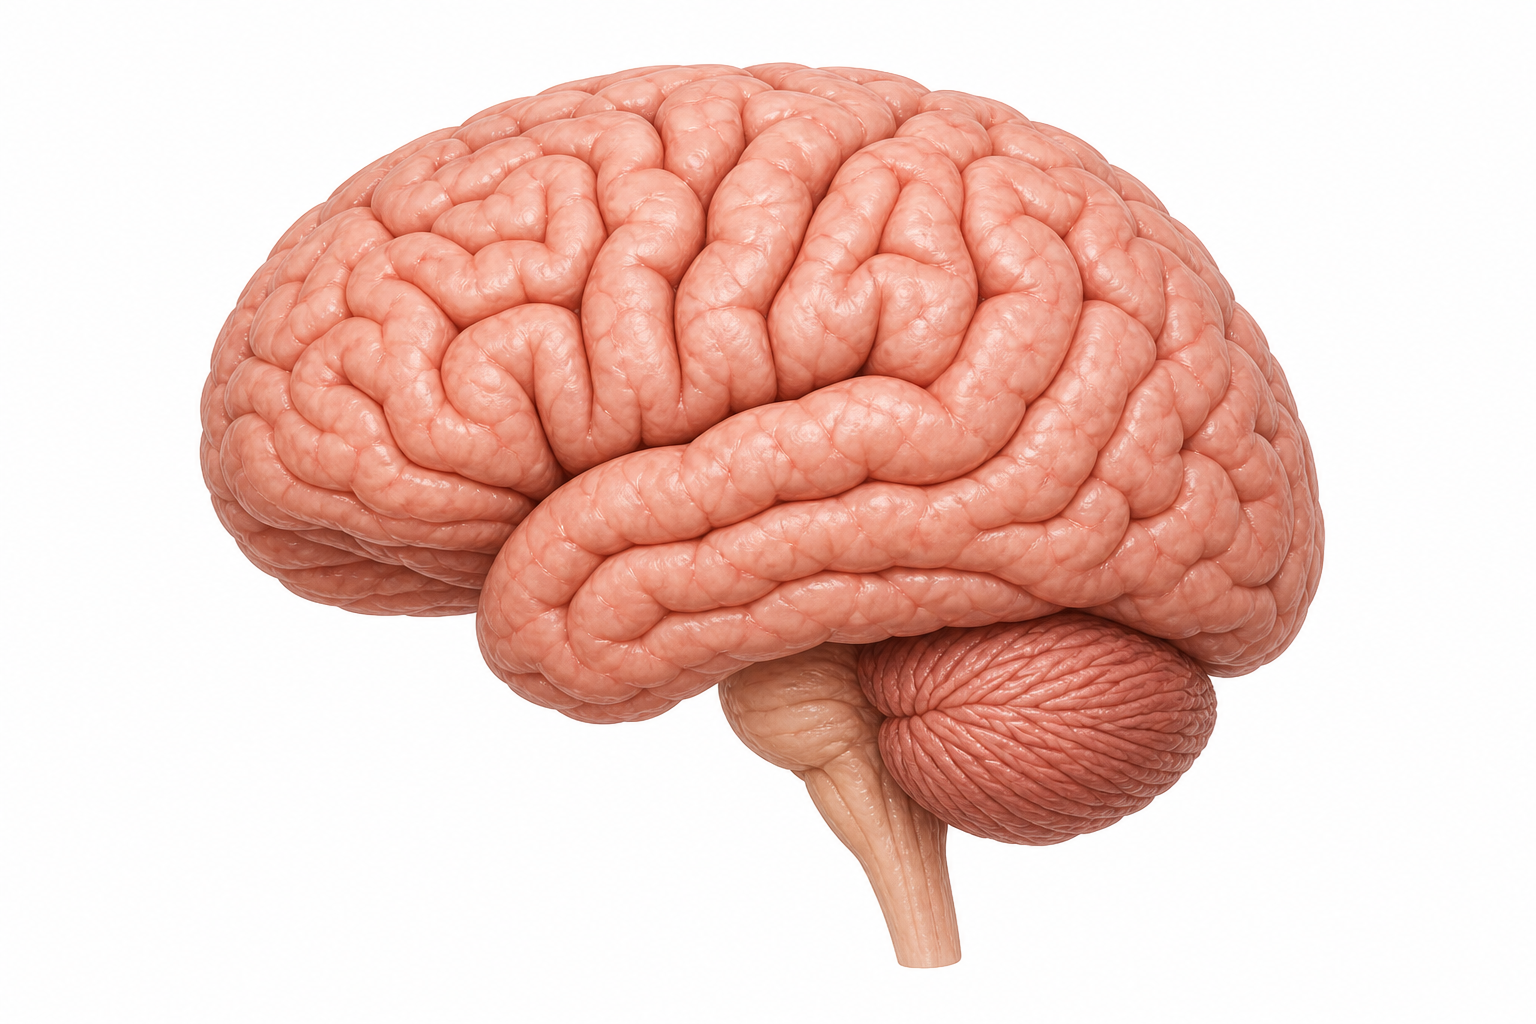
\includegraphics[width=0.52\linewidth]{images/book2/ai/fig-brain-side.png}};
  \begin{scope}[x={(img.south east)}, y={(img.north west)},
      every node/.style={font=\small}]
    \draw[omDef, thick] (0.85,0.55) -- (1.05,0.70) node[right, align=left] {primaire visuele schors\\ (achterhoofdskwab)};
    \draw[omDef, thick] (0.70,0.75) -- (0.80,1.06) node[above] {wandbeenkwab};
    \draw[omDef, thick] (0.28,0.72) -- (0.20,1.06) node[above] {voorhoofdskwab};
    \draw[omDef, thick] (0.48,0.42) -- (0.40,-0.06) node[below] {slaapkwab};
    \draw[omDef, thick] (0.70,0.28) -- (1.05,0.20) node[right] {kleine hersenen};
  \end{scope}
\end{tikzpicture}

{\small De hersenen van de linkerkant gezien. De \omterm{prop:g11:vision-and-brain:pathway}{primaire visuele schors}
ligt helemaal achterin, in de achterhoofdskwab; de verdere visuele
gebieden strekken zich daarvandaan naar voren uit, de slaapkwab in (wat
de dingen zijn) en de wandbeenkwab in (waar zij zijn en hoe zij bewegen).}
\end{omfigure}

\section{Vele gebieden, één waarneming}

\begin{proposition}[Gespecialiseerde visuele gebieden]\label{prop:g11:vision-and-brain:areas}
De \omterm{prop:g11:vision-and-brain:pathway}{primaire visuele schors} geeft haar analyse door aan een tiental verdere
\emph{visuele gebieden}, elk met een eigen specialisme: het ene haalt de
kleur eruit, het andere de beweging, weer andere vorm, diepte, gezichten,
geschreven woorden. Hun uitkomsten worden --- samen met het geheugen en
met de andere zintuigen --- samengevoegd tot de ene samenhangende
waarneming die wij ervaren. Die waarneming is een bouwsel: de hersenen
vullen de blinde vlek op, maken verborgen contouren af, houden kleuren
constant onder wisselend licht, en zijn te misleiden door
gezichtsbedrog dat hun regels uitbuit.
\end{proposition}
\begin{proof}[Bewijsmateriaal]
Plaatselijke beschadigingen halen de onderdelen uit elkaar: een patiënt
met schade aan het kleurgebied ziet een grijze wereld met een normale
gezichtsscherpte; schade aan het bewegingsgebied laat kleur en vorm gaaf
maar heft de waarneming van beweging op; schade aan een gebied van de
slaapkwab heft alleen het herkennen van gezichten op. Beeldvorming van de
werking bij gezonde vrijwilligers laat dezelfde gebieden oplichten, het
ene voor gekleurde patronen, het andere voor bewegende stippen, weer een
ander voor gezichten, terwijl de primaire schors op alle reageert.
Elektroden bij dieren vinden in elk gebied neuronen die op de eigenschap
van dat gebied reageren en op weinig anders.
\end{proof}

\begin{omfigure}
\begin{tikzpicture}[font=\small, >=Stealth,
  b/.style={draw, rounded corners, align=center, text width=2.5cm, minimum height=1.0cm}]
  \node[b, fill=omDef!12] (ret) at (0,0) {netvlies:\\ licht wordt signaal};
  \node[b, fill=omDef!12] (v1) at (3.6,0) {primaire visuele\\ schors: randen,\\ richtingen, kaart};
  \node[b, fill=omProp!15] (col) at (7.4,1.6) {kleurgebied};
  \node[b, fill=omProp!15] (mov) at (7.4,0) {bewegingsgebied};
  \node[b, fill=omProp!15] (shp) at (7.4,-1.6) {gebieden voor vorm\\ en gezichten};
  \node[b, fill=omMeth!15, text width=2.8cm] (per) at (11.2,0) {waarneming:\\ één tafereel, met\\ geheugen erbij};
  \draw[->, thick] (ret) -- (v1);
  \draw[->, thick] (v1) -- (col); \draw[->, thick] (v1) -- (mov); \draw[->, thick] (v1) -- (shp);
  \draw[->, thick] (col) -- (per); \draw[->, thick] (mov) -- (per); \draw[->, thick] (shp) -- (per);
\end{tikzpicture}

{\small Van signalen tot een tafereel. De primaire schors verdeelt haar
analyse over gespecialiseerde gebieden waarvan de uitkomsten weer worden
samengevoegd. Een beschadiging in één gebied neemt één eigenschap weg ---
kleur, beweging, gezichten --- en laat de rest staan.}
\end{omfigure}

\begin{example}[Drie patiënten, drie gebieden]\label{ex:g11:vision-and-brain:patients}
De patiënte die in grijs ziet, heeft aan beide kanten een beschadiging van
het kleurgebied; de \omterm{def:g11:the-eye:photoreceptors}{kegeltjes} van haar netvlies werken, en haar primaire
schors ontvangt hun signalen, maar de fase die verhoudingen tussen
\omterm{def:g11:the-eye:photoreceptors}{kegeltjes} in kleur omzet, is weg. De patiënte die geen beweging ziet,
heeft het bewegingsgebied verloren: zij ziet opeenvolgende
momentopnamen. De patiënte die geen gezichten herkent, heeft een
beschadiging van het gezichtengebied van de slaapkwab; zij herkent mensen
aan hun stem of aan een hoed. In elk geval is wat verloren gaat nauwkeurig
begrensd, en wat overblijft laat zien dat de andere gebieden op eigen
kracht werken.
\end{example}

\section{Een schors die door ervaring wordt gebouwd}

\begin{proposition}[Plasticiteit]\label{prop:g11:vision-and-brain:plasticity}
De verbindingen van de \omterm{prop:g11:vision-and-brain:pathway}{visuele schors} liggen bij de geboorte niet vast.
Tijdens een \emph{gevoelige periode} vroeg in het leven worden zij gevormd
door wat de ogen zien; bij de volwassene blijven zij veranderen, maar
trager, door leren en gebruik. Die \emph{hersenplasticiteit}\index{hersenplasticiteit}
is een eigenschap van neuronen: verbindingen die worden gebruikt, worden
versterkt en vermenigvuldigd; verbindingen die niet worden gebruikt,
worden verzwakt en gesnoeid.
\end{proposition}
\begin{proof}[Bewijsmateriaal]
Hubel en Wiesel (jaren zestig) namen metingen op uit de \omterm{prop:g11:vision-and-brain:pathway}{visuele schors} van
katten en apen. Bij een normaal dier reageren de meeste neuronen op beide
ogen. Bij een dier waarvan één oog de eerste maanden gesloten werd
gehouden, reageert vrijwel elk neuron alleen op het open oog: de
verbindingen van het gesloten oog zijn overgenomen. Het oog van een
volwassen dier even lang sluiten verandert niets. Bij mensen houdt een
kind van wie één oog sterk onscherp of scheef staat en dat niet vóór
ongeveer het zevende jaar wordt behandeld, blijvend een zwak oog ---
amblyopie --- hoe goed de optiek later ook is. Bij volwassenen vergroot
het leren lezen van braille het schorsgebied voor de lezende vinger; het
leren jongleren vergroot de gebieden die beweging verwerken, en die
krimpen weer als het oefenen ophoudt.
\end{proof}

\begin{omfigure}
\begin{tikzpicture}
\begin{axis}[
  ybar, bar width=9pt,
  width=0.86\linewidth, height=5.6cm,
  axis x line=bottom, axis y line=left,
  ymin=0, ymax=60, ylabel={neuronen in de schors (\%)},
  ylabel style={font=\small},
  symbolic x coords={alleen links, vooral links, beide gelijk, vooral rechts, alleen rechts},
  xtick=data, tick label style={font=\small},
  xlabel={welk oog het neuron aanstuurt},
  xlabel style={font=\small, at={(axis description cs:0.5,-0.16)}, anchor=north},
  enlarge x limits=0.15, ytick={0,20,40,60},
  legend style={at={(0.5,-0.34)}, anchor=north, legend columns=2, font=\small, draw=none},
]
\addplot[fill=omDef!50, draw=omDef] coordinates {(alleen links,12) (vooral links,20) (beide gelijk,36) (vooral rechts,20) (alleen rechts,12)};
\addplot[fill=omThm!50, draw=omThm] coordinates {(alleen links,2) (vooral links,3) (beide gelijk,5) (vooral rechts,30) (alleen rechts,60)};
\legend{normaal katje, katje met het linkeroog drie maanden gesloten}
\end{axis}
\end{tikzpicture}

{\small De bevinding van Hubel en Wiesel, afgerond. Bij een normaal katje
antwoorden de meeste neuronen van de \omterm{prop:g11:vision-and-brain:pathway}{visuele schors} op beide ogen. Na drie
maanden met het linkeroog gesloten antwoorden negen van de tien neuronen
alleen nog op het rechteroog: de verbindingen van het ongebruikte oog zijn
verloren gegaan.}
\end{omfigure}

\begin{example}[Waarom scheelzien vroeg moet worden behandeld]\label{ex:g11:vision-and-brain:amblyopia}
Een kind van drie met één naar binnen gedraaid oog ziet dubbel, en de
hersenen onderdrukken het zwakkere beeld. Wordt het oog niet rechtgezet,
of het goede oog niet enkele uren per dag afgeplakt om het zwakke aan het
werk te zetten, dan bouwt de schors zich tijdens de gevoelige periode rond
het goede oog om, en blijft het zwakke oog, hoe optisch volmaakt ook, zijn
leven lang blind voor fijne details. Op zijn derde behandeld herstelt het
kind zijn volle zicht; op zijn twaalfde behandeld vrijwel niet.
\end{example}

\section{Drugs en de ziende hersenen}

\begin{proposition}[Neuronen, boodschappers, en moleculen die hen nabootsen]\label{prop:g11:vision-and-brain:drugs}
Neuronen praten met elkaar bij \emph{synapsen} door chemische
boodschappers, \emph{neurotransmitters}, op de receptoren van de volgende
\omterm{def:g10:cells-common-unit:cell}{cel} los te laten; het laatste jaar beschrijft dat mechanisme. Verscheidene
neurotransmitters, waaronder \emph{serotonine}, regelen de stroom van
signalen door de visuele gebieden. Moleculen waarvan de vorm op een
neurotransmitter lijkt, kunnen zich aan zijn receptoren binden en die
stroom verstoren: lyserginezuurdi-ethylamide (LSD) bindt zich aan
serotoninereceptoren in de \omterm{prop:g11:vision-and-brain:pathway}{visuele schors} en brengt hallucinaties voort
--- kleuren, vormen en bewegingen die worden gezien zonder dat er licht
bij hoort. Zulke middelen kunnen blijvende veranderingen achterlaten:
episodes die maanden later terugkeren, en bij sommige mensen aanhoudende
stoornissen in het zien.
\end{proposition}
\admitted

\begin{example}[Wat een hallucinatie laat zien]\label{ex:g11:vision-and-brain:hallucination}
Onder LSD is het netvlies onveranderd en brengt de primaire schors nog
altijd in kaart wat de ogen zien; de verstoring zit in de latere gebieden
en in de manier waarop zij worden samengevoegd. Er verschijnen patronen
die op de eigen bouwstenen van de schors lijken --- roosters, spiralen,
tunnels --- omdat het middel de machinerie van de waarneming laat draaien
zonder haar invoer. De hallucinatie is een demonstratie, door het
haperen, dat het zien door de hersenen wordt gemaakt en dat een molecuul
het kan veranderen.
\end{example}

\begin{method}[Een stoornis in het zien lokaliseren]\label{met:g11:vision-and-brain:locate}
\begin{enumerate}
  \item Eén oog blind, het andere normaal: het oog of zijn oogzenuw,
        vóór de kruising.
  \item Beide ogen blind voor dezelfde helft van het veld: de
        tegenoverliggende oogzenuwbaan, thalamus of primaire schors.
  \item Beide ogen blind voor de buitenste helften van het veld: de
        kruising, waar de overstekende vezels zijn doorgesneden.
  \item Het zien gaaf maar één eigenschap weg (kleur, beweging,
        gezichten): het bijbehorende gespecialiseerde gebied.
  \item De waarneming verstoord bij normale ogen en normale schors, en
        van voorbijgaande aard: een middel of een stofwisselingsoorzaak.
\end{enumerate}
\end{method}

\begin{remark}[Wat dit jaar heeft laten zien]\label{rem:g11:vision-and-brain:year}
Het oog van \cref{ch:g11:the-eye} was een zaak van \omterm{def:g10:universal-dna:gene}{genen} en \omterm{def:g10:chemistry-of-life:families}{eiwitten}:
\omterm{def:g11:the-eye:photoreceptors}{opsines}, hun verdubbelingen, een kleurenblindheid die via de X wordt
geërfd. De hersenen van dit hoofdstuk zijn een zaak van verbindingen, door
gebruik gevormd. Daartussen ligt het hele onderwerp van dit jaar --- van
de volgorde van een \omterm{def:g10:universal-dna:gene}{gen} tot een kenmerk, en van het kenmerk tot wat een
mens kan --- en de les dat bij elke stap het \omterm{def:g11:enzymes-and-phenotype:phenotype}{genotype} voorstelt en de
omgeving, van de temperatuur van de oren van een kat tot het licht dat het
oog van een katje ontvangt, beschikt.
\end{remark}

\section{Oefeningen}

\begin{exercise}[$\star$]\label{exo:g11:vision-and-brain:1}
Volg de weg van een signaal uit de linkerhelft van het gezichtsveld naar
de schors.
\end{exercise}

\begin{exercise}[$\star$]\label{exo:g11:vision-and-brain:2}
Wat gebeurt er bij de oogzenuwkruising, en welke vezels steken over?
\end{exercise}

\begin{exercise}[$\star$]\label{exo:g11:vision-and-brain:3}
Noem drie gespecialiseerde visuele gebieden en het uitvalsverschijnsel dat
een beschadiging van elk oplevert.
\end{exercise}

\begin{exercise}[$\star$]\label{exo:g11:vision-and-brain:4}
Definieer \omterm{prop:g11:vision-and-brain:plasticity}{hersenplasticiteit} en de gevoelige periode.
\end{exercise}

\begin{exercise}[$\star$]\label{exo:g11:vision-and-brain:5}
Hoe werkt LSD op het visuele stelsel in?
\end{exercise}

\begin{exercise}[$\star\star$]\label{exo:g11:vision-and-brain:6}
Lokaliseer met \cref{met:g11:vision-and-brain:locate} de beschadiging bij
een patiënt die met beide ogen blind is voor de rechterhelft van het veld.
\end{exercise}

\begin{exercise}[$\star\star$]\label{exo:g11:vision-and-brain:7}
Een \omterm{def:g11:cancer:cancer}{tumor} drukt van onderen op de oogzenuwkruising en snijdt de
overstekende vezels door. Welke delen van het veld verliest de patiënt?
Leg dat uit met de figuur.
\end{exercise}

\begin{exercise}[$\star\star$]\label{exo:g11:vision-and-brain:8}
Welk deel van de neuronen reageert volgens de figuur van Hubel en Wiesel
überhaupt op het linkeroog, bij het normale katje en bij het beroofde?
\end{exercise}

\begin{exercise}[$\star\star$]\label{exo:g11:vision-and-brain:9}
Waarom behandelt het enkele uren per dag afplakken van het goede oog van
een scheelziend kind de amblyopie? Waarom faalt dezelfde behandeling bij
een volwassene?
\end{exercise}

\begin{exercise}[$\star\star$]\label{exo:g11:vision-and-brain:10}
Leg uit waarom de patiënte die in grijs ziet niet kleurenblind is in de
zin van \cref{ch:g11:the-eye}, en hoe een test de twee aandoeningen zou
kunnen onderscheiden.
\end{exercise}

\begin{exercise}[$\star\star$]\label{exo:g11:vision-and-brain:11}
Het schorsgebied voor de vingers van een pianiste is groter dan
gemiddeld. Leg dat uit met plasticiteit, en zeg wat je voorspelt als zij
jarenlang niet meer speelt.
\end{exercise}

\begin{exercise}[$\star\star\star$]\label{exo:g11:vision-and-brain:12}
Bij iemand die door staar blind is geboren, wordt die op haar dertigste
weggenomen. Voorspel met de gevoelige periode wat zij de eerste weken
ziet en wat zij wel en niet zal terugkrijgen.
\end{exercise}

\begin{exercise}[$\star\star\star$]\label{exo:g11:vision-and-brain:13}
Leg met de verdeling van de zintuigcellen en de ganglioncellen uit
\cref{ch:g11:the-eye} uit waarom de kaart in de schors meer oppervlak aan
het midden van het veld toekent dan aan de rand.
\end{exercise}

\begin{exercise}[$\star\star\star$]\label{exo:g11:vision-and-brain:14}
Beeldvorming van de werking laat het kleurgebied actief zien wanneer een
proefpersoon zich met gesloten ogen een rode appel voorstelt. Wat zegt dat
over het verband tussen de gespecialiseerde gebieden en de waarneming, en
over hallucinaties?
\end{exercise}

\begin{exercise}[$\star\star\star$]\label{exo:g11:vision-and-brain:15}
"Het zien wordt door het oog gedaan." Herschrijf die uitspraak correct in
een alinea, met de drie patiënten, de katjes en het middel.
\end{exercise}

\section{Probleem: Vier patiënten en een katje}

\begin{problem}[{Weekendprobleem --- stoornissen in het zien
gelokaliseerd langs de baan, een schors in kaart gebracht door prikkeling,
de beroving van een katje geteld, en het scheelzien van een kind op tijd
behandeld}]
\label{pb:g11:vision-and-brain:1}
Er worden vier patiënten onderzocht. A: blind aan het linkeroog, het
rechteroog normaal. B: met beide ogen blind voor de linkerhelft van het
veld. C: met beide ogen blind voor de buitenste helft van hun veld (het
linkeroog naar links, het rechteroog naar rechts). D: normale velden,
normale gezichtsscherpte, maar geen waarneming van beweging.

\medskip
\noindent\textbf{Deel I --- Lokaliseren.}
\begin{enumerate}
  \item Lokaliseer de beschadiging van A. Welke structuur, en vóór of na
        de kruising?
  \item Lokaliseer de beschadiging van B, en zeg waarom zij na de
        kruising moet liggen.
  \item Lokaliseer de beschadiging van C nauwkeurig, met uitleg welke
        vezels zijn doorgesneden.
  \item Lokaliseer de beschadiging van D. Wat zegt het behoud van velden
        en gezichtsscherpte je over de primaire schors?
  \item Zeg voor elke patiënt of het netvlies gaaf is, en hoe je dat zou
        nagaan.
\end{enumerate}

\medskip
\noindent\textbf{Deel II --- De kaart.}
Tijdens een operatie geeft het prikkelen van punten van de rechter \omterm{prop:g11:vision-and-brain:pathway}{visuele
schors} van een patiënt flitsen. Prikkeling van de punt van de
achterhoofdskwab geeft een flits in het midden van het veld; punten verder
naar voren geven flitsen verder naar buiten in het linkerveld;
\qty{1}{cm} schors bij de punt bestrijkt ongeveer $2^\circ$ van het veld,
terwijl \qty{1}{cm} verder naar voren $20^\circ$ bestrijkt.
\begin{enumerate}[resume]
  \item Waarom liggen alle flitsen in het linkerveld?
  \item Hoeveel schors vertegenwoordigt de centrale $2^\circ$ vergeleken
        met een band van $2^\circ$ op $40^\circ$ van het midden? Bereken
        de verhouding.
  \item Breng die verhouding in verband met de gele vlek en de rand van
        het netvlies.
  \item Een kleine beschadiging bij de punt van de rechter
        achterhoofdskwab: wat verliest de patiënt? En een beschadiging van
        dezelfde omvang verder naar voren?
  \item Waarom kan de patiënt met de kleine centrale beschadiging toch
        nog lezen, zij het langzaam, door zijn ogen te bewegen?
\end{enumerate}

\medskip
\noindent\textbf{Deel III --- Het katje.}
Uit de figuur van Hubel en Wiesel.
\begin{enumerate}[resume]
  \item Welk percentage van de neuronen reageert bij het normale katje in
        enige mate op beide ogen?
  \item Welk percentage reageert bij het beroofde katje überhaupt op het
        gesloten (linker)oog?
  \item Het netvlies en de oogzenuw van het gesloten oog zijn gaaf. Waar
        is zijn invoer gebleven, en wat heeft de ruimte ingenomen?
  \item Dezelfde sluiting bij een volwassen kat verandert niets. Wat
        stelt dat vast, en wat is de menselijke tegenhanger ervan?
  \item Bij een katje worden beide ogen drie maanden gesloten. Voorspel
        het histogram en het zicht van het dier daarna.
\end{enumerate}

\medskip
\noindent\textbf{Deel IV --- Het kind.}
Een kind van vier heeft een naar binnen gedraaid linkeroog; de optiek
ervan is normaal. Onbehandeld neemt de schors de invoer van het
rechteroog over.
\begin{enumerate}[resume]
  \item Leg met het katje uit wat er met het zicht van het linkeroog
        gebeurt als er niets wordt gedaan, en waarom een bril alleen dat
        niet voorkomt.
  \item De behandeling is om het \emph{rechteroog} maandenlang enkele
        uren per dag af te plakken. Leg uit waarom juist het goede oog
        wordt afgedekt.
  \item Waarom moet dat vóór ongeveer het zevende jaar gebeuren, en
        waarom faalt dezelfde behandeling op het vijftiende?
  \item Een volwassene die op zijn dertigste een oog verliest, raakt de
        schors die eraan gewijd was niet op dezelfde manier kwijt. Breng
        dat in overeenstemming met het katje.
  \item Geef het resultaat: de vier beschadigingen gelokaliseerd van voor
        naar achter langs de baan, en de ene eigenschap van de schors ---
        met naam --- die de behandeling van het kind alleen op tijd laat
        werken.
\end{enumerate}
\end{problem}
